\documentclass[pdflatex,ja=standard,fleqn]{bxjsarticle}
\usepackage{ascmac,amsmath,amssymb,type1cm,graphicx}
\title{材料力学レポート1}
\author{J4-210447 川村朋広}
\begin{document}
\maketitle
\begin{itembox}[l]{課題}
    図のような鉄筋コンクリート梁の鉄筋量が$100$から$6000mm^2$まで、変化した場合の梁の曲げ耐力$P$の変化を、指定のコンクリートの強度ごとに計算する。\\
    鉄筋量をx軸に、曲げ耐力をy軸にとりグラフを作成する。なお条件は以下の通りとする。\\\\
    コンクリートの圧縮強度は以下の場合を考える\\
    \quad$f^{\prime}_{c}=25$MPa,$35$Mpa,$45$Mpa
\end{itembox}
\begin{figure}[htbp]
    \centering
    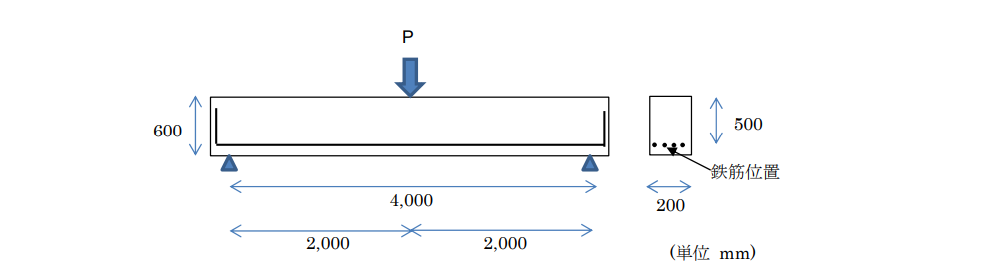
\includegraphics[width=15cm]{2023-01-15.png}
\end{figure}
\begin{table*}[htbp]
    \centering
    \begin{tabular}{clll}
         & 変数名 & 値 & 単位\\ \hline
        コンクリートの終局ひずみ & $\epsilon^{\prime}_{cu}$ & $0.0035$ & \\
        コンクリートの合力 & $C$ & & MPa\\
        鉄筋の降伏応力 & $f_{sy}$ & $450$ & MPa\\
        鉄筋の降伏ひずみ & $\epsilon_{sy}$ & & MPa\\
        ヤング率 & $E_{s}$ & 200,000 & MPa\\
        鉄筋量 & $A_{s}$ & & $mm^2$\\
        鉄筋の合力 & $T$ & & MPa\\
        つり合い鉄筋比 & $P_{b}$ & & \\
        断面の横の長さ & $b$ & $200$ & mm\\
        断面の有効高さ & $d$ & $500$ & mm\\
        中立軸までの高さ & $x$ & & mm
    \end{tabular}
\end{table*}
\section{つり合い鉄筋比を求める}
ひずみ分布の傾きが中立軸の上下で一致することから
\begin{align*}
    &\frac{\epsilon^{\prime}_{cu}}{x}=\frac{\epsilon_{sy}}{d-x}\\
    &\frac{x}{d}=\frac{\epsilon^{\prime}_{cu}}{\epsilon^{\prime}_{cu}+\epsilon_{sy}}
\end{align*}
となる。また、鉄筋の合力とコンクリートの合力がつりあうとき
\begin{eqnarray*}
    T&=&C\\
    &=&A_{s}f_{sy}\\
    &=&0.85f^{\prime}_{c}\times 0.8x\times b
\end{eqnarray*}
が成り立つ。さらに鉄筋の降伏ひずみは
\begin{eqnarray*}
    \epsilon_{sy}=\frac{f_{sy}}{E_{s}}=0.00225
\end{eqnarray*}
以上よりつり合い鉄筋比$P_{b}$は
\begin{eqnarray*}
    P_{b}&=&\frac{A_{s}}{bd}\\
    &=&\frac{1}{bd}\frac{T}{f_{sy}}\\
    &=&\frac{0.85f^{\prime}_{c}\times 0.8x\times b}{bdf_{sy}}\\
    &=&\frac{0.68f^{\prime}_{c}}{f_{sy}}\frac{x}{d}\\
    &=&\frac{0.68\epsilon^{\prime}_{cu}}{\epsilon^{\prime}_{cu}+\epsilon_{sy}}\frac{f^{\prime}_{c}}{f_{sy}}
\end{eqnarray*}
で求められる。なお、ここでの$A_{s}$は釣り合う時の鉄筋量に過ぎない。\\
それぞれのケースにおけるつり合い鉄筋比は以下の通りとなった。
\begin{table*}[htbp]
    \begin{tabular}{ccc}
        $f_{sy}$ & $P_{b}$ \\\hline
        $25$MPa & 0.0379 & \\
        $35$MPa & 0.0530 & \\
        $45$MPa & 0.0682 &
    \end{tabular}
\end{table*}
\section{鉄筋量$A_{s}$と曲げ耐力$P$の関係を求める}
鉄筋比は
\begin{eqnarray*}
    p=\frac{A_{s}}{bd}=\frac{A_{s}}{1.0\times 10^5}
\end{eqnarray*}
となる。
\subsection{$p<P_{b}$のとき}
梁は曲げ引張破壊を引き起こす。この時、中立軸は
\begin{eqnarray*}
    x=\frac{A_{s}f_{sy}}{0.68\times f^{\prime}_{c}\times b}
\end{eqnarray*}
となる。したがって破壊時の曲げモーメント$M_{u}$は
\begin{eqnarray*}
    M_{u}&=&A_{s}f_{sy}(d-0.4x)\\
    &=&A_{s}f_{sy}(d-0.4\times \frac{f_{sy}}{0.68\times f^{\prime}_{c}\times b}A_{s})
\end{eqnarray*}
となるので、破壊時荷重は梁の長さ$L$を用いて
\begin{eqnarray*}
    P&=&\frac{4M_{u}}{L}\\
    &=&\frac{4f_{sy}}{L}A_{s}(d-0.4\times \frac{f_{sy}}{0.68\times f^{\prime}_{c}\times b}A_{s})
\end{eqnarray*}
となり$A_{s}$に関する2次曲線となる。
\subsection{$p>P_{b}$のとき}
梁は曲げ圧縮破壊を起こす。コンクリート応力と鉄筋応力の力のつり合いより
\begin{eqnarray*}
    T&=&A_{s}E_{s}\epsilon_{s}\\
    &=&0.85f^{\prime}_{c}\times 0.8x\times b
\end{eqnarray*}
また、ひずみ分布の傾きが中立軸の上下で一致することから
\begin{eqnarray*}
    \epsilon_{s}=\frac{d-x}{x}\epsilon^{\prime}_{cu}
\end{eqnarray*}
これらを$x$について解くと、
\begin{eqnarray*}
    x=\frac{k}{2}(\sqrt{1+\frac{4d}{k}}-1)
\end{eqnarray*}
となる。なお、定数$k$を以下のように定義した。
\begin{eqnarray*}
    k=\frac{A_{s}E_{s}\epsilon^{\prime}_{cu}}{0.68\times f^{\prime}_{c}\times b}
\end{eqnarray*}
この時、破壊時の曲げモーメントは
\begin{eqnarray*}
    M_{u}=0.85f^{\prime}_{c}\times 0.8x\times b\times (d-0.4x)
\end{eqnarray*}
となるから、破壊時の荷重は、
\begin{eqnarray*}
    P&=&\frac{4M_{u}}{L}\\
    &=&\frac{4\times 0.85f^{\prime}_{c}\times 0.8x\times b}{L}(d-0.4x)
\end{eqnarray*}
となる。\\
この関係を用いてグラフにプロットしていくと以下のようなグラフとなった。横軸の単位$mm^2$で縦軸の単位はkNである。
\begin{figure}[htbp]
    \centering
    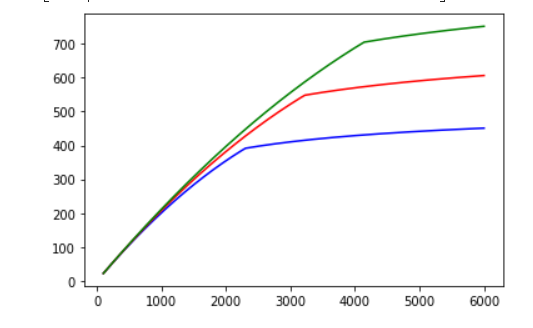
\includegraphics[width=10cm]{2023-01-16.png}
\end{figure}
\end{document}